\documentclass{article}
\usepackage{tikz}
\usepackage{pgfplots}
\usepackage{pdfpages}
\usepackage{fontspec}
\usetikzlibrary{decorations.text,pgfplots.groupplots,intersections}
\pgfplotsset{compat=1.7}

\definecolor{nice_blue}{HTML}{377EB8}
\definecolor{nice_green}{HTML}{4DAF4A}
\definecolor{nice_purple}{HTML}{984EA3}
\definecolor{nice_red}{HTML}{E41A1C}
\definecolor{nice_orange}{HTML}{FF7F00}
\definecolor{nice_pink}{HTML}{FB9A99}

\pgfplotsset{
    simple graphs/.style={
        domain=0:12
        ,xmin=0
        ,xmax=12
        ,ymin=0
        ,ymax=12
        ,axis lines*=left
        ,xtick=\empty
        ,ytick=\empty
        ,every axis y label/.style={
            at={(axis description cs:0.09,.5)}
            ,rotate=90
            ,anchor=south},
        }
        ,every axis x label/.style={
            at={(axis description cs:0.5,-0.1)}
            ,anchor=south}
        }

\begin{document}
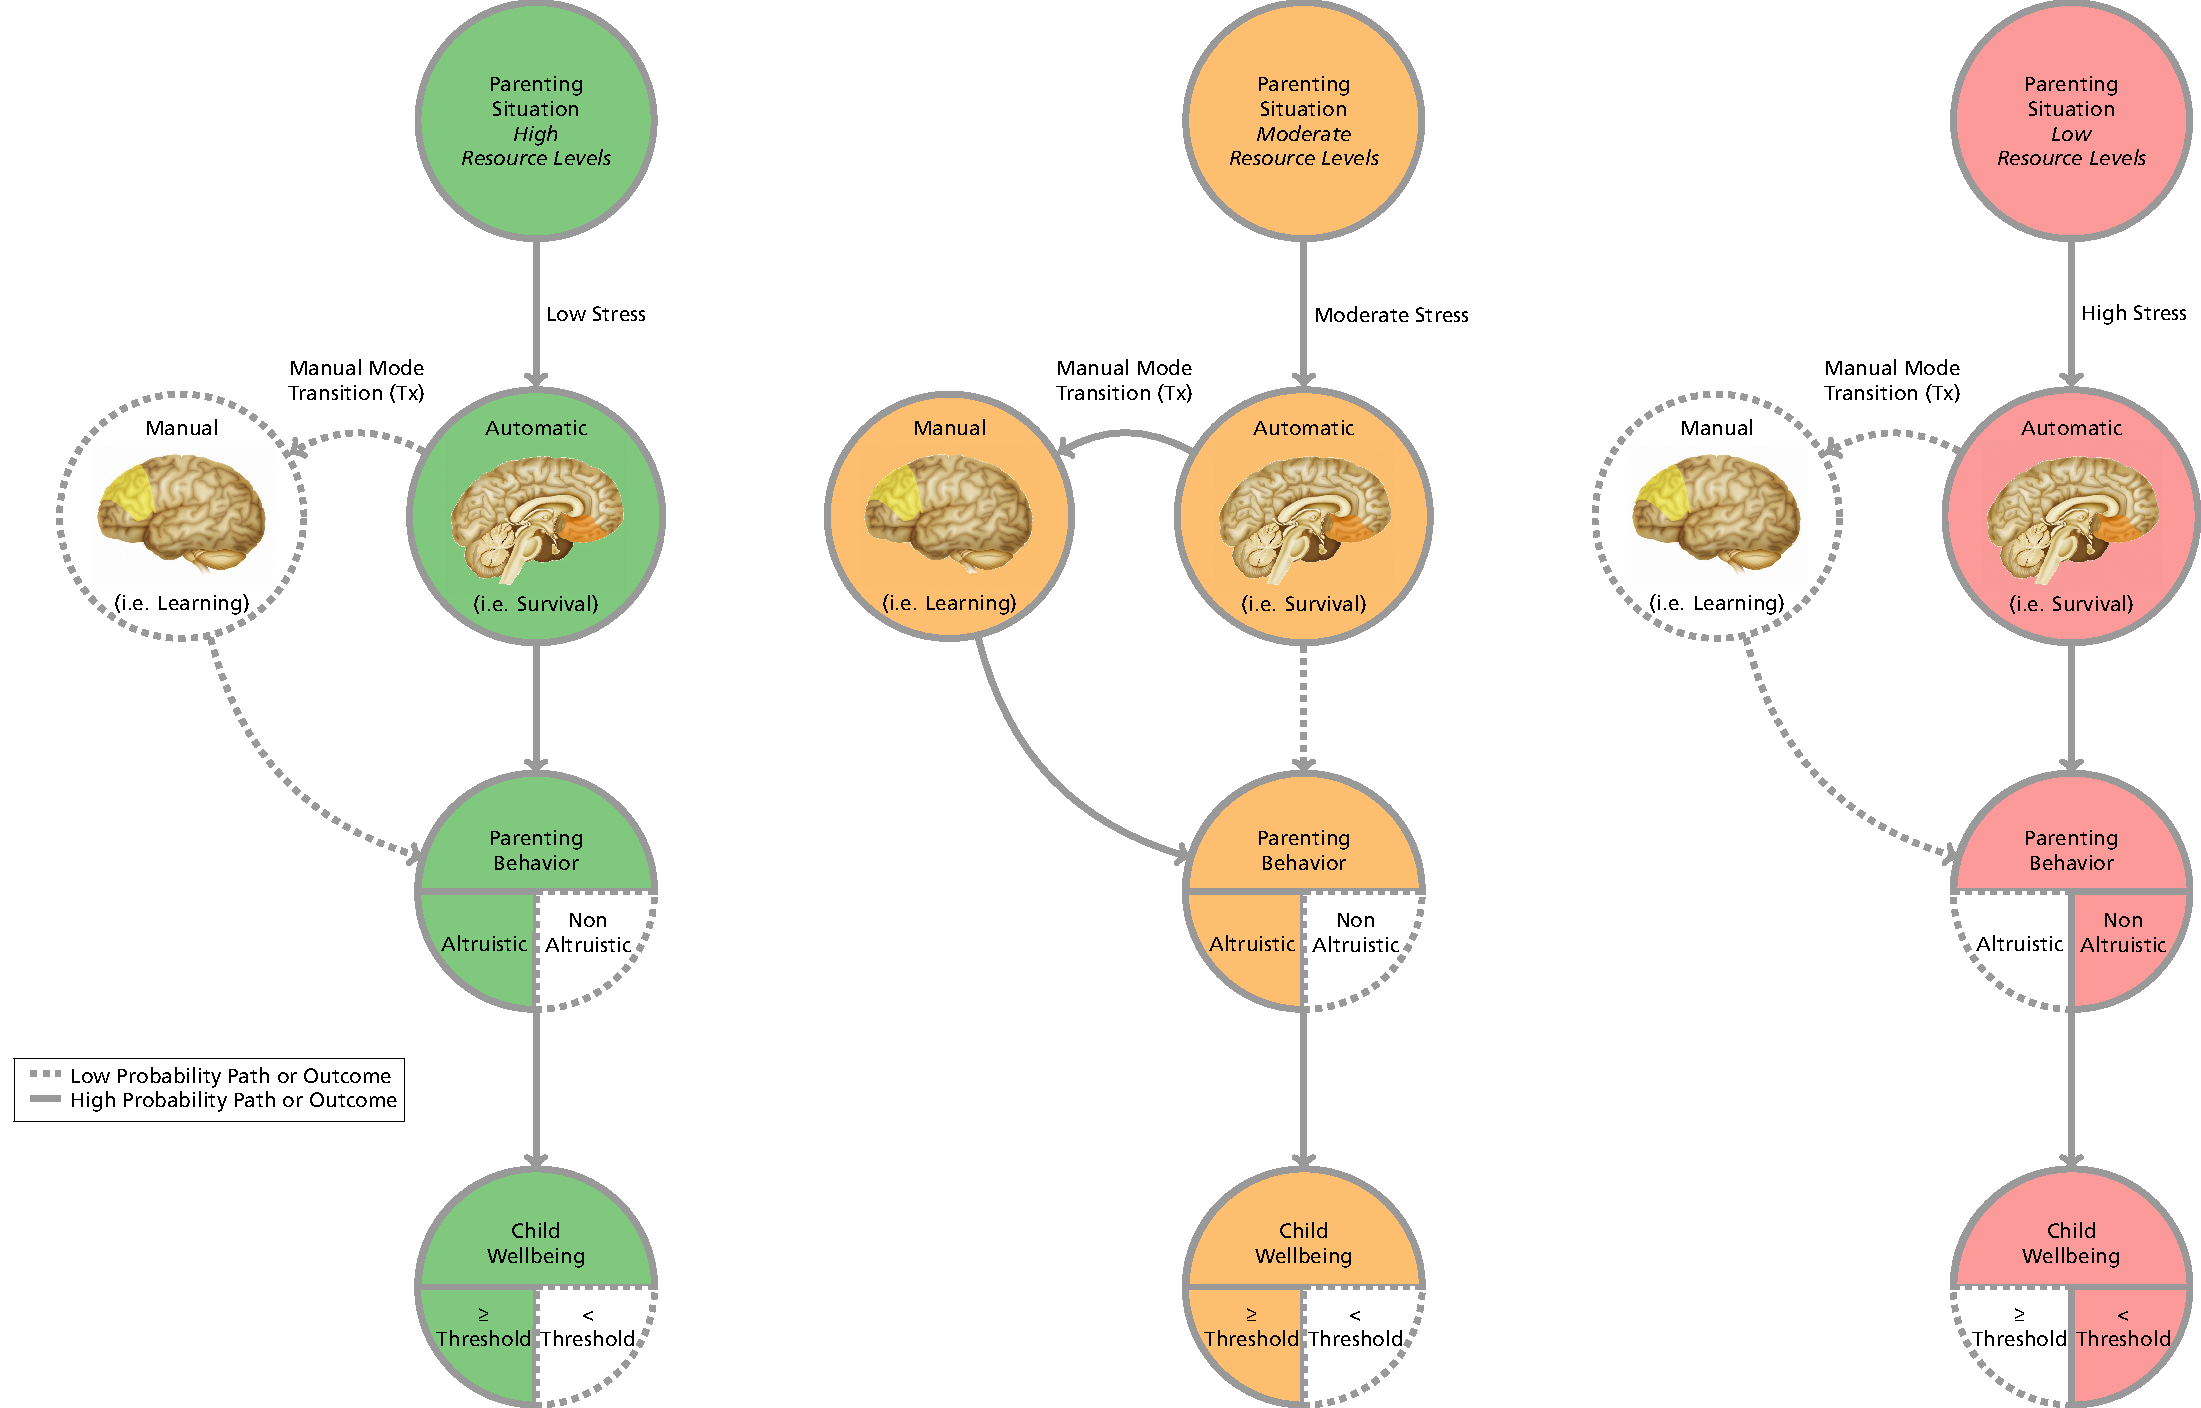
\includepdf[scale=0.95,pages={1},landscape=true,pagecommand=\section{title}]{general_conceptual_model_flow.pdf}

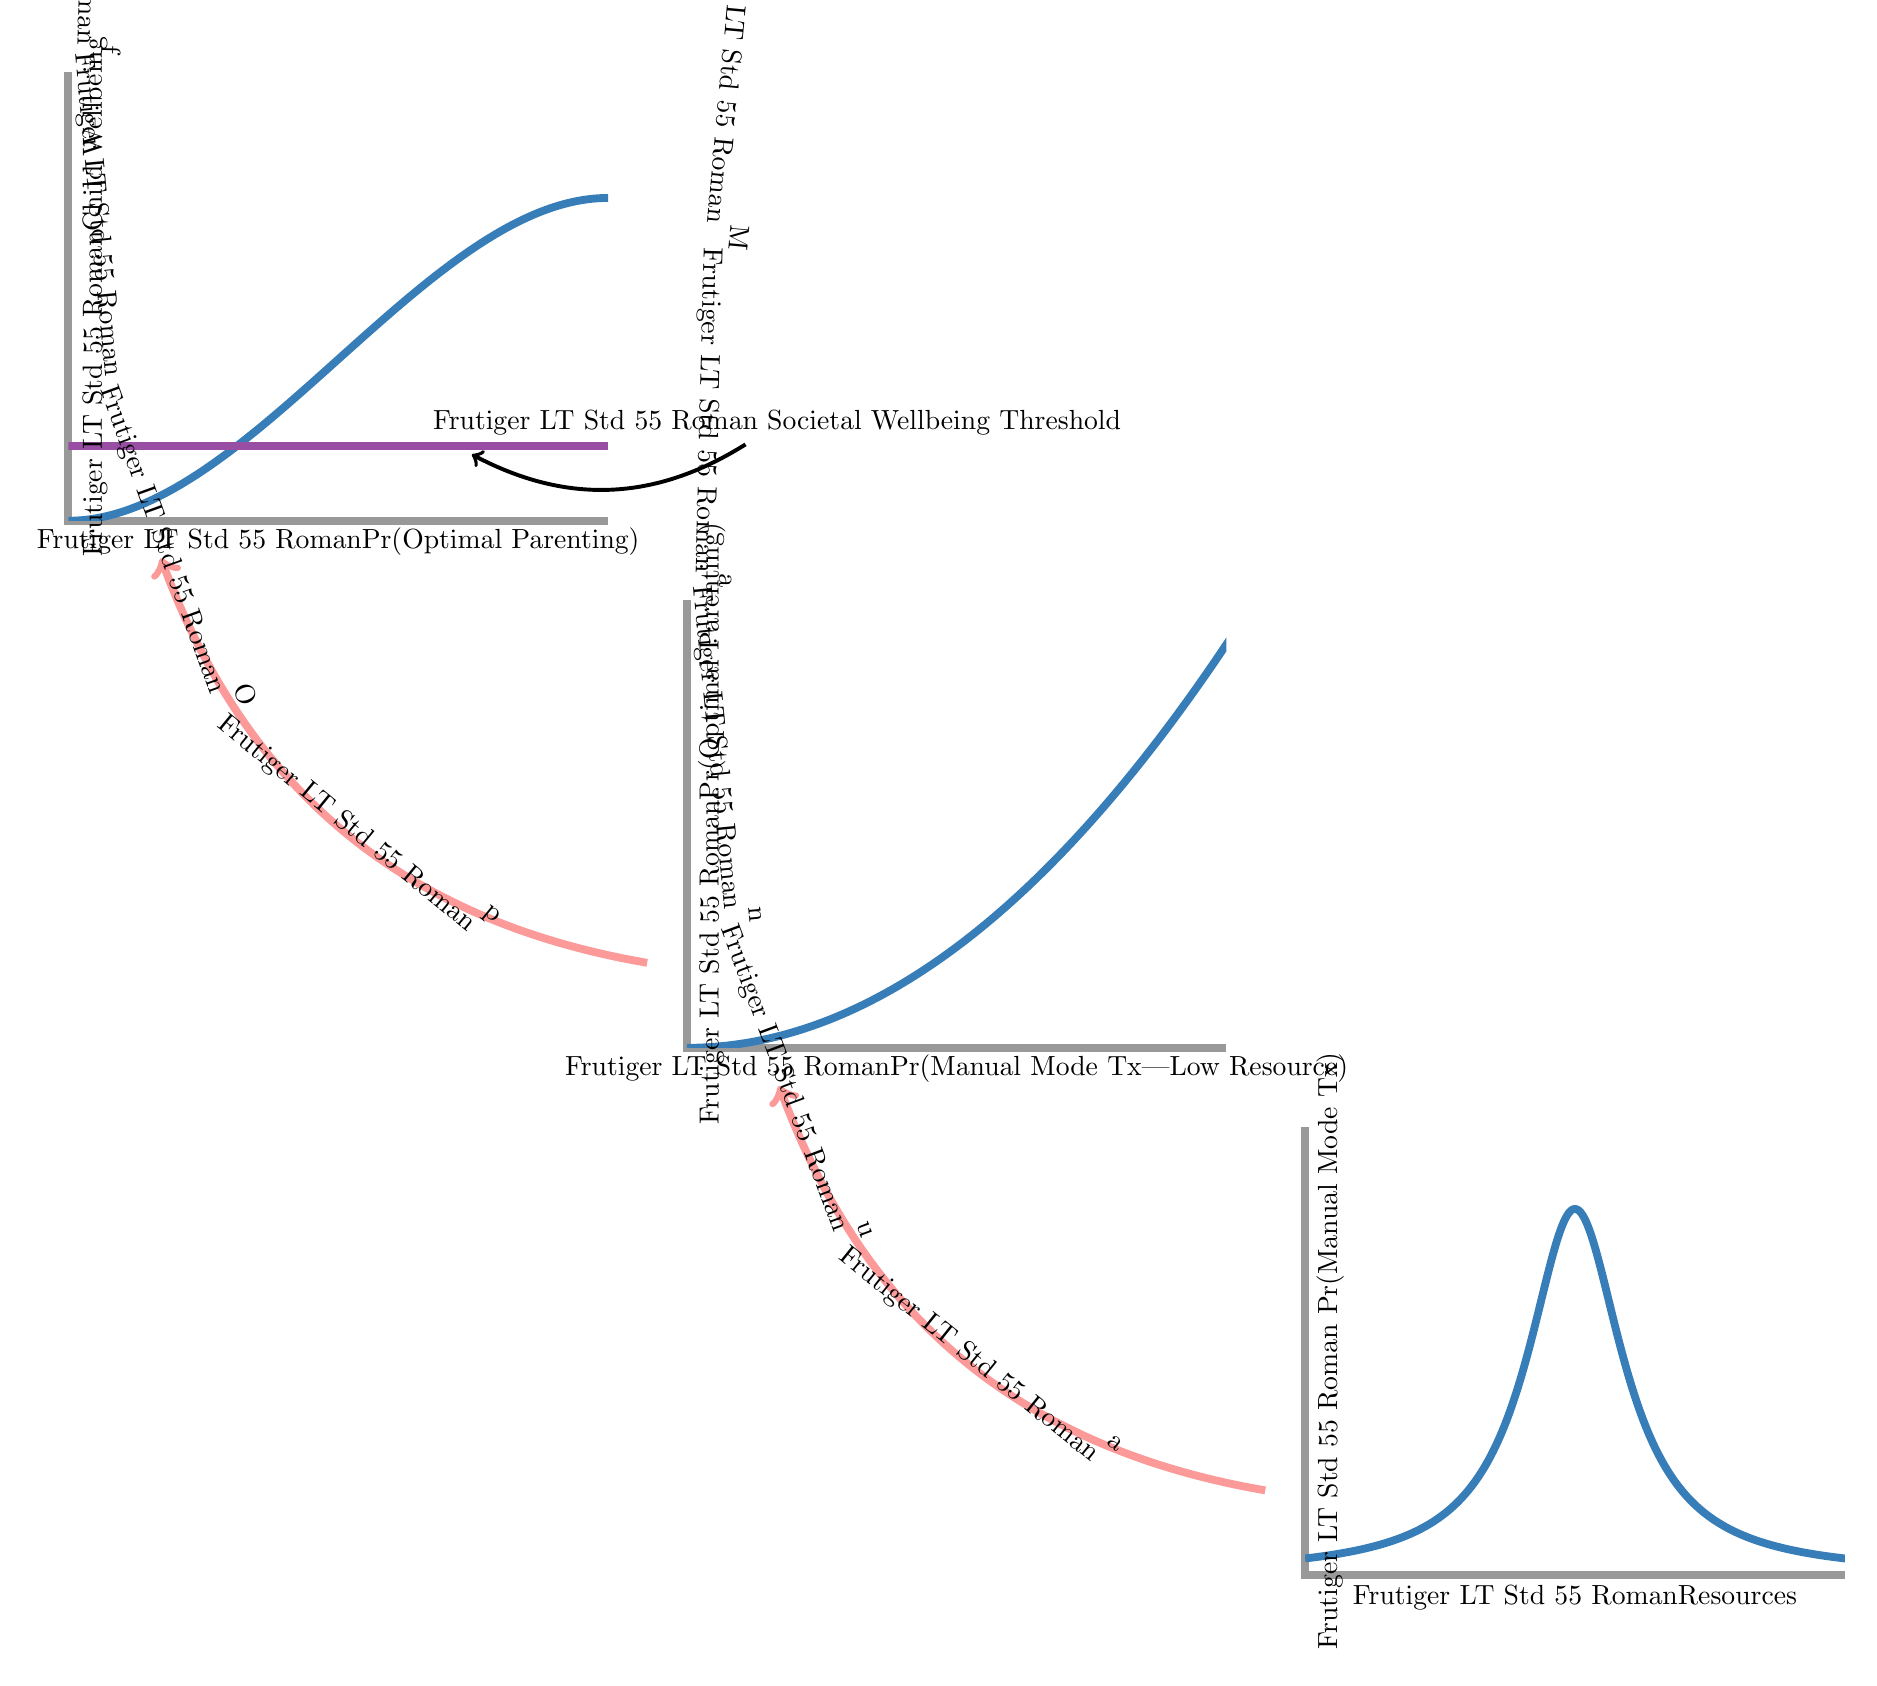
\begin{tikzpicture}

\def\myshift#1{\raisebox{2ex}}

\centering

% %start of mal optimal parenting
% \coordinate (a1o1) at (0,0);
% %end of mal optimal parenting
% \coordinate (a2o1) at (1,0);
% %start of mal manual mode
% \coordinate (a1m1) at (7.85,-6.7);
% %end of mal manual mode
% \coordinate (a2m1) at (7.85,-5.7);
% %start of normal optimal parenting
% \coordinate (n1o1) at (6.85,0);
% %start of normal manual mode
% \coordinate (n1m1) at (7.85,-1);


%\filldraw[nice_red!70] (a1m1) to [bend left, auto] (a1o1) -- (a2o1) to [bend right, auto] (a2m1);
%\filldraw[nice_purple!70] (a2o1) to [bend right, auto] (a2m1) -- (n1m1) to [bend left, auto] (n1o1);
%
% %start of mal optimal parenting
% \coordinate (a1o2) at (0+7.85,0-6.7);
% %end of mal optimal parenting
% \coordinate (a2o2) at (1+7.85,0-6.7);
% %start of mal manual mode
% \coordinate (a1m2) at (7.85+7.85,-6.7-6.7);
% %end of mal manual mode
% \coordinate (a2m2) at (7.85+7.85,-5.7-6.7);
% %start of normal optimal parenting
% \coordinate (n1o2) at (6.85+7.85,0-6.7);
% %start of normal manual mode
% \coordinate (n1m2) at (7.85+7.85,-1-6.7);

\node (OPy) at (7.85,-5.7) [draw=none,circle,minimum size=10mm,inner sep=0mm] {};
\node (MMx) at (7.85+1,-6.7) [draw=none,circle,minimum size=10mm,inner sep=0mm] {};

\node (MMy) at (7.85+7.85,-5.7-6.7) [draw=none,circle,minimum size=10mm,inner sep=0mm] {};
\node (OPx) at (1,0) [draw=none,circle,minimum size=10mm,inner sep=0mm] {};

\node (wbar) at (9,1.25) [draw=none,fill=none] {\fontspec{Frutiger LT Std 55 Roman} Societal Wellbeing Threshold};
\node (wbar_arrow_end) at (5,.9) [draw=none,fill=none] {};

\draw[->,bend left, line width=2.83464567*0.5pt]  (wbar) to node [auto] {} (wbar_arrow_end);

\begin{groupplot}[
    group style={
        group size=3 by 3,
    },
    simple graphs,
    ytick=\empty,
    xtick=\empty,
    enlarge x limits=false,
    axis lines*=left,
    axis line style = {gray!80, line width=2.83464567pt,shorten <=-0.5\pgflinewidth}
]



\nextgroupplot[ymax=6
              ,xmax=6
              ,ylabel=\fontspec{Frutiger LT Std 55 Roman}Child Wellbeing
              ,xlabel=\fontspec{Frutiger LT Std 55 Roman}Pr(Optimal Parenting)
              ]
\addplot[->
        ,nice_blue
        ,line width=2.83464567pt
        ,samples=1000]
        {2*(.18*x^2 - .02*x^3)};

\addplot[nice_purple, line width=2.83464567pt] plot coordinates {
        (0,1)
        (6,1)};

\nextgroupplot[hide y axis, hide x axis]
%empty plot spec
\nextgroupplot[hide y axis, hide x axis]
%empty plot spec
\nextgroupplot[hide y axis, hide x axis]
%empty plot spec

\nextgroupplot[ymax=6
              ,xmax=6
              ,ylabel=\fontspec{Frutiger LT Std 55 Roman}Pr(Optimal Parenting)
              ,xlabel=\fontspec{Frutiger LT Std 55 Roman}Pr(Manual Mode Tx|Low Resource)
              ]
\addplot[->
        ,nice_blue
        ,line width=2.83464567pt
        ,samples=1000]
        {.15*x^2};


\nextgroupplot[hide y axis, hide x axis]
%empty plot spec
\nextgroupplot[hide y axis, hide x axis]
%empty plot spec
\nextgroupplot[hide y axis, hide x axis]
%empty plot spec


\nextgroupplot[ymax=.6
               ,xmax=6
               ,ylabel=\fontspec{Frutiger LT Std 55 Roman} Pr(Manual Mode Tx)
               ,xlabel=\fontspec{Frutiger LT Std 55 Roman}Resources
               ]

\addplot[->
          ,nice_blue
          ,line width=2.83464567pt
          ,samples=1000]
          {(1/pi)*(.65/((x-3)^2 + .65^2))};

\end{groupplot}F

\draw[<-
      ,name path = abuse_start
      ,bend right
      ,nice_pink
      ,line width=2.83464567pt
      ,postaction={decorate
                    ,decoration={text along path
                                ,text align=center
                                ,text={|\fontspec{Frutiger LT Std 55 Roman}\myshift|Low Levels of Optimal Parenting}}}
      ]  (OPx) to node [auto] {} (OPy);

\draw[<-
      ,name path = abuse_start
      ,bend right
      ,nice_pink
      ,line width=2.83464567pt
      ,postaction={decorate
                    ,decoration={text along path
                                ,text align=center
                                ,text={|\fontspec{Frutiger LT Std 55 Roman}\myshift|Low Levels of Manual Mode Cognitition}}}
      ]  (MMx) to node [auto] {} (MMy);

\end{tikzpicture}
\end{document}
